\documentclass{beamer}
\usepackage{graphicx}
\graphicspath{ {./images/} }

\title{WaterWizards}
\author{Justin Dewitz, Max Kondratov, Erick Zeiler, Julian <Nachname>}
\date{17. Juli 2025}

\begin{document}

\frame{\titlepage}

\begin{frame}
\frametitle{Inhaltsverzeichnis}
\tableofcontents
\end{frame}

\section{Einleitung}
\begin{frame}
\frametitle{Einleitung}
\begin{itemize}
  \item Was ist WaterWizards?
  \begin{enumerate}
    \item Mulitplayer Real-Time Schiffe versenken
    \item Angriff durch Zauber, die durch Karten repräsentiert werden
    \item Ziel: Zerstörung der gegnerischen Schiffe
  \end{enumerate}
  \item Warum WaterWizards?
  \begin{enumerate}
    \item Schiffe versenken ist ein Klassiker
    \item Durch Real-Time wird es dynamischer
    \item Für jede Altersgruppe interessant
  \end{enumerate}
  \item Was macht WaterWizards besonders?
    \begin{enumerate}
      \item Kombination aus Strategie und schnellen Entscheidungen
      \item Zauber und Karten bringen neue Dynamik ins Spiel
      \item Multiplayer und Echtzeit sorgen für Spannung
    \end{enumerate}
  \item Für wen ist das Spiel gedacht?
    \begin{enumerate}
      \item Strategie-Fans
      \item Familien und Freunde
      \item Alle Altersgruppen
    \end{enumerate}
\end{itemize}
\end{frame}

\section{Organisation}
\begin{frame}
  \frametitle{Organisation}
  \begin{itemize}
    \item git über GitHub für die Versionsverwaltung 
    \item Scrum mit 2-Wochen-Sprints
    \item Kanban/Issue-Board über GitHub
    \item Kommunikation über Discord-Server
  \end{itemize}
\end{frame}

\section{Rollen des Projektes}
\begin{frame}
\frametitle{Rollen des Projektes}

\end{frame}

\subsection{Ansprechpartner}
\begin{frame}
\frametitle{Ansprechpartner}

\end{frame}

\section{Technologie + Architektur}
\begin{frame}
\frametitle{Technologie + Architektur}
  \begin{itemize}
    \item Programiersprache: C\#
    \item Raylib für die grafische Darstellung
    \item LiteNetLib für die Client-Server-Verbindung
    \item Nuke für das Build-System
    \item CodeQl für die statische Code-Analyse
    \item GitHub Actions für die CD-Pipeline
    \item GitHub Pages für die Dokumentation
    \item Event-Driven Architektur
    \item Docker für die Containerisierung
    \item Hetzner Server für das Hosting
  \end{itemize}
\end{frame}

\subsection{UI}
\begin{frame}
  \frametitle{UI}
  \begin{itemize}
    \item Raylib für die grafische Darstellung
    \item GameScreen als Hauptkomponente
    \item GameBoard für die Spielbretter
    \item GameShip für die Schiffe
    \item GameCard für die Karten
    \item GameHand für die Hand der Spieler
  \end{itemize} 
\end{frame}

\subsection{GameScreen}
\begin{frame}
\frametitle{GameScreen}
  \begin{itemize}
    \item GameScreen enthält alles, was auf dem Bildschirm gezeigt wird
      \begin{enumerate}
        \item Die beiden Spielbretter (GameBoard) mit Schiffen (GameShip) und Steinen
        \item Die Karten (GameCard) auf der Hand (GameHand) der Spieler
        \item Die Kartenstapel (CardStack) der einzelnen Kartentypen (CardType)
      \end{enumerate}
  \end{itemize}
  
\end{frame}


\subsection{Server/Backend}
\begin{frame}
\frametitle{Server/Backend}
  \begin{itemize}
    \item Das Backend ist in C\# mit der Library LiteNetLib geschrieben
    \item Ein globaler Server der eine Lobby auf Hetzner bereitstellt
    \item Server wird in Docker-Containern ausgeführt
  \end{itemize}
\end{frame}

\subsection{Shared}
\begin{frame}
\frametitle{Shared}
  \begin{itemize}
    \item Shared enthält alle Klassen, die sowohl im Client als auch im Server verwendet werden
    \item Enthält die Definitionen der Karten und der Kartentypen
    \item Enthält die Definitionen der Schiffe und der Schiffs-Typen
  \end{itemize}
\end{frame}

\subsection{Backend - Client Kommunikation}
\begin{frame}
\frametitle{Backend - Client Kommunikation}
\begin{columns}
  \begin{column}{0.45\textwidth}
    Event-Driven Architektur
    \begin{itemize}
      \item UDP für die Echtzeit-Kommunikation
      \item Nachrichten basiertes Protokoll für beidseitige Kommunikation
    \end{itemize}
  \end{column}
  \begin{column}{0.55\textwidth}
    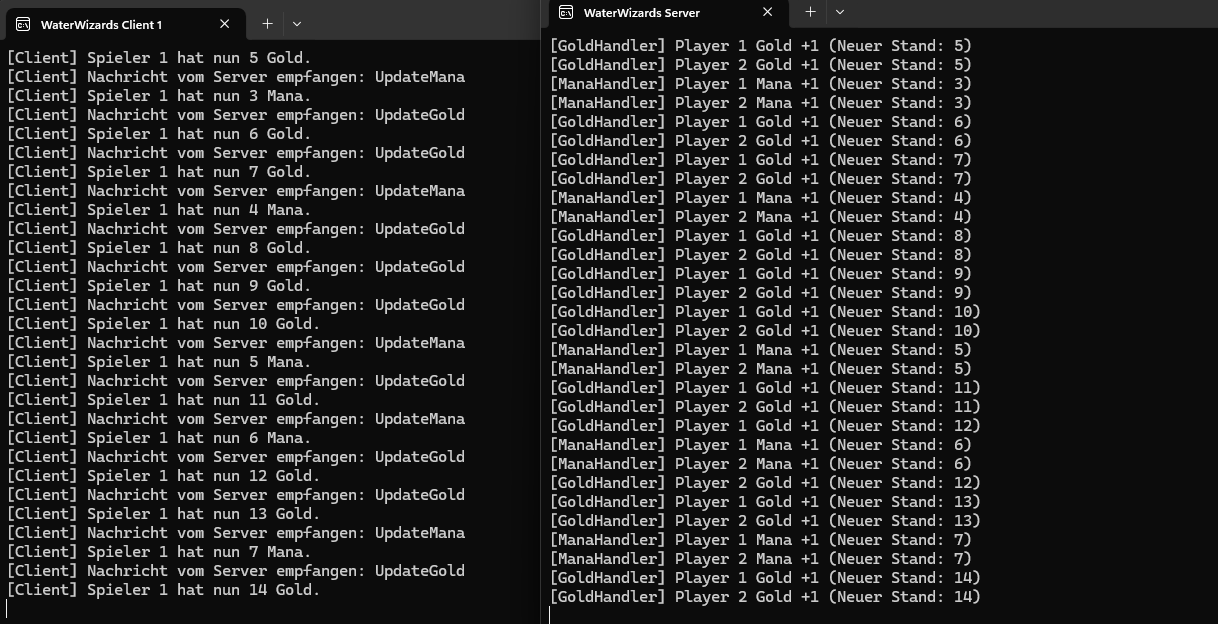
\includegraphics[width=\textwidth]{Server-Client-Logs.png}
  \end{column}
\end{columns}
\end{frame}

\section{Technische Erfahrungen}
\begin{frame}
\frametitle{Technische Erfahrungen}
\end{frame}

\section{Analyse}
\begin{frame}
\frametitle{Analyse}
\begin{columns}
  \begin{column}{1\textwidth}
    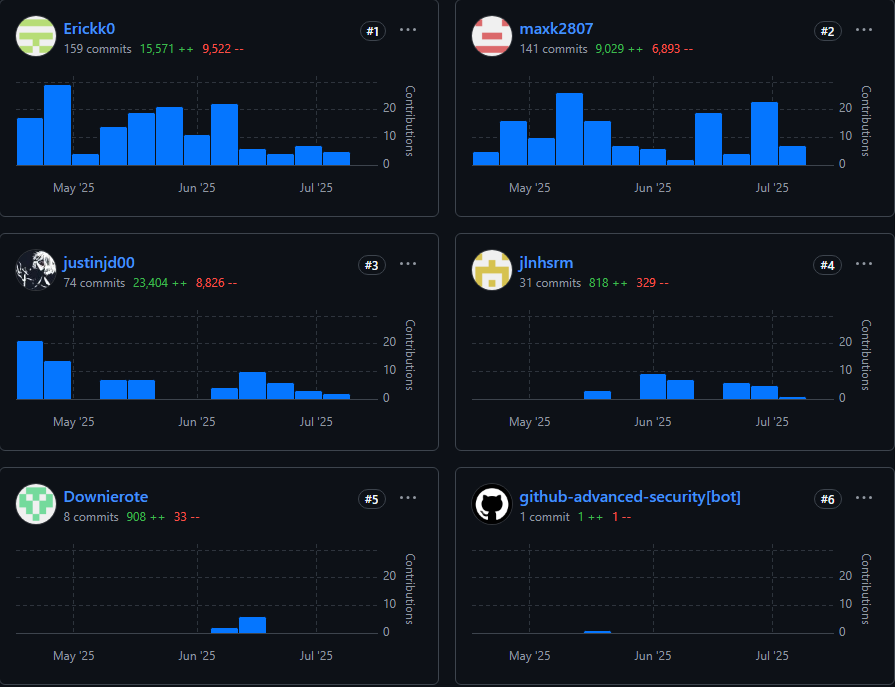
\includegraphics[width=\textwidth]{GitHub-Insights.png}
  \end{column}
\end{columns}
\end{frame}

\section{Wiki}
\begin{frame}
\frametitle{Wiki}

\end{frame}

\section{Erfahrungen und Fazit}
\begin{frame}
\frametitle{Erfahrungen und Fazit}

\end{frame}


\end{document}